% !TeX spellcheck = en_GB
\documentclass{beamer}\mode<presentation>{\usetheme{AMSCesenaPurpleAndGold}}
\setbeamertemplate{bibliography item}{\insertbiblabel}

\usepackage{common}

\newcommand{\labN}{2}

\title[L\labN{} -- \jade{} Exercises]{L\labN{} -- \jade{} in Practice}
%
\subtitle[SD]{Distributed Systems / Technologies}
%
\author[Ciatto \and Omicini]
{\emph{Giovanni Ciatto} \and Andrea Omicini\\
\texttt{giovanni.ciatto@unibo.it \and andrea.omicini@unibo.it}}
%
\institute[DISI, Univ. Bologna]
{Dipartimento di Informatica -- Scienza e Ingegneria (DISI)\\\textsc{Alma Mater Studiorum} -- Universit{\`a} di Bologna a Cesena}
%
\date[A.Y. 2020/2021]{Academic Year 2020/2021}

\setbeamercovered{transparent}

\AtBeginSection{
    \begin{frame}[c]\frametitle{Outline}
        % 		\begin{multicols}{2}
        \tableofcontents[sectionstyle=show/shaded, subsectionstyle=show/shaded, subsubsectionstyle=hide/hide]
        % 		\end{multicols}
    \end{frame}
}

\AtBeginSubsection{
    \begin{frame}[c]\frametitle{Next in Line\ldots}
        % 		\begin{multicols}{2}
        \tableofcontents[sectionstyle=shaded/shaded, subsectionstyle=show/shaded, subsubsectionstyle=hide/hide]
        % 		\end{multicols}
    \end{frame}
}

\begin{document}

\maketitle

%\section{Motivation}

%\begin{frame}[allowframebreaks]
%\frametitle{Motivation}
%
%    \begin{itemize}
%        \item Some motivation
%
%    \end{itemize}
%
%\end{frame}

% \begin{frame}
% \frametitle{Lecture goals}

%     \begin{itemize}
%         \item some goals
%     \end{itemize}

% \end{frame}

%===============================================================================
\section{\jade{} Basics}
%===============================================================================

%-------------------------------------------------------------------------------
\subsection{\jade{} Architecture}
%-------------------------------------------------------------------------------

%\\\\\\\\\\\\\\\\\\\\\
\begin{frame}[c,allowframebreaks]\frametitle{\jade{} Architecture: Recap}
    %
    \begin{center}
        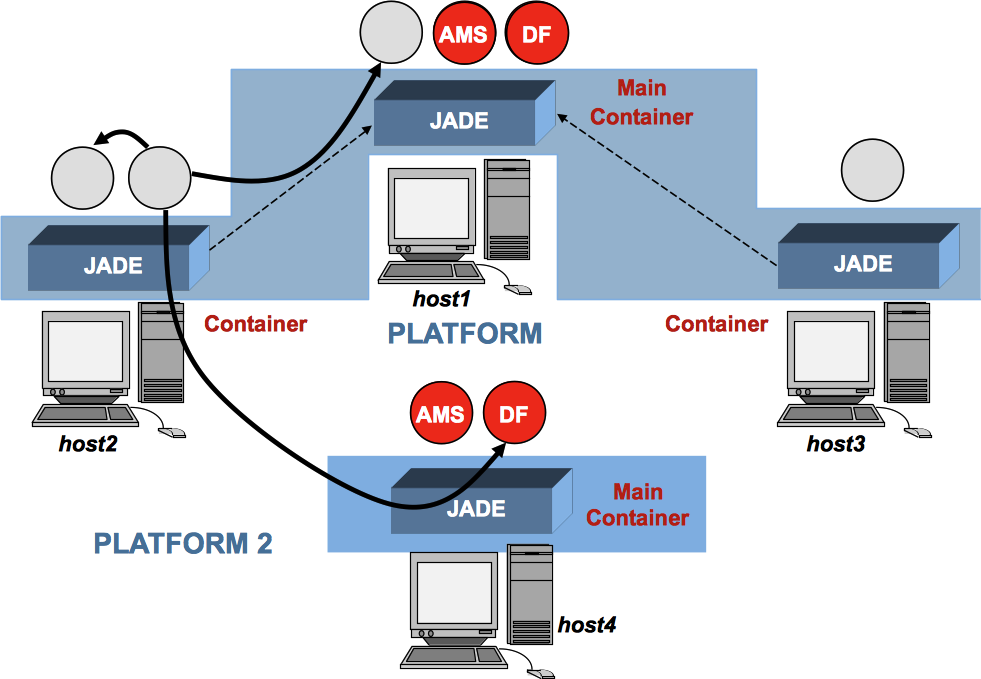
\includegraphics[width=.75\textwidth]{res/img/jade_archi}
    \end{center}
    %
    \begin{block}{Containers}
        %
        \begin{itemize}
            \item \alert{agents runtimes}, the \emph{environments} without which agents cannot exist
            \item \emph{one} main container for \emph{each} \jade{} platform\ldots
            \item \ldots{} but many peripheral containers may coexist in the same platform and in the same host too
            \item they automatically register themselves to the (default/given) main container
            \item one single JVM executed per host/platform (2 \jade{} on the same host are 2 JVM)
        \end{itemize}
        %
    \end{block}
    %
    \begin{block}{Agent Management System (AMS)}
        %
        \begin{itemize}
            \item \jade{} \alert{white pages} service
            \item \emph{one} AMS service (agent) for \emph{each} \jade{} platform
            \item always runs in the main container
            \item is contacted (automatically) by every \jade{} agent upon start\ldots
            %
            \begin{itemize}
                \item AMS \texttt{register()} method called prior to agent \texttt{setup()} abstract method being called by the container
            \end{itemize}
            %
            \item \ldots and death
            %
            \begin{itemize}
                \item \texttt{deregister()} called after \texttt{takedown()}
            \end{itemize}
            %
        \end{itemize}
        %
    \end{block}
    %
    \begin{block}{Agent Communication Channel (ACC)}
        %
        \begin{itemize}
            \item \jade{} \emph{distributed, location-transparent} \alert{messaging service}
            \item \alert{asynchronous} by default (uncoupling for agents autonomy)
            \item also supporting \emph{synchronous communication}, if required
            \item compliant to \fipa{} \acl{} message format
        \end{itemize}
        %
    \end{block}
    %
    \begin{block}{Directory Facilitator (DF)}
        %
        \begin{itemize}
            \item \jade{} \alert{yellow pages} service
            \item similar to the AMS agent
            %
            \begin{itemize}
                \item \emph{one} DF service (agent) for \emph{each} \jade{} platform
                \item always runs in the main container
            \end{itemize}
            %
            \item except that it should be explicitly contacted by \emph{advertising} and \emph{client} agents upon need---\emph{public/subscribe} pattern
        \end{itemize}
        %
    \end{block}
    %
\end{frame}
%\\\\\\\\\\\\\\\\\\\\\

%-------------------------------------------------------------------------------
\subsection{\jade{} Agents}
%-------------------------------------------------------------------------------

%\\\\\\\\\\\\\\\\\\\\\
\begin{frame}\frametitle{\jade{} Agents: Recap}
    %
    \begin{block}{\jade{} agents}
        %
        \begin{itemize}
            \item instances of \alert{\texttt{jade.core.Agent}}-derived classes
            \item \alert{single-threaded}, \emph{multitasking} computational model based on concurrent behaviours
            \item \emph{asynchronous} communication model based on \fipa{} \acl{} messages
            \item FSM-like lifecycle with public methods to perform state transitions
            \item \texttt{jade.core.AID} class implements the globally unique naming service
            %
            \begin{itemize}
                \item agent name of the kind \texttt{<localname>@<platformname>}
                \item pool of platform addresses, only used for \emph{inter-platform} communications
            \end{itemize}
            %
        \end{itemize}
        %
    \end{block}
    %
\end{frame}
%\\\\\\\\\\\\\\\\\\\\\

%\\\\\\\\\\\\\\\\\\\\\
\begin{frame}[c]\frametitle{Agents Lifecycle}
    %
    \begin{block}{Lifecycle methods}
        %
        \begin{description}
            \item[\texttt{doActivate()}] from SUSPENDED to where it was when \texttt{doSuspend()} was called
            \item[\texttt{doDelete()}] from either state to UNKNOWN
            \item[\texttt{doWait()}] from ACTIVE to WAITING
            \item[\texttt{doSuspend()}] from ACTIVE or WAITING to SUSPENDED
            \item[\texttt{doWake()}] from WAITING to ACTIVE
            \item[\texttt{doMove()}] from either state to TRANSIT
            \item[\texttt{doClone()}] same as \texttt{doMove()}
        \end{description}
        %
    \end{block}
    %
\end{frame}
%\\\\\\\\\\\\\\\\\\\\\

%\\\\\\\\\\\\\\\\\\\\\
\begin{frame}[c,allowframebreaks]\frametitle{Agents Execution}
    %
    \begin{block}{Starting agents}
        Agents are launched with command
        %
        \begin{center}
            \texttt{java -cp \ldots{} jade.Boot \ldots{} -agents <name>:<class>}
        \end{center}
        %
        (or, from the RMA GUI)
        %
        \begin{enumerate}
            \item the agent constructor is executed
            \item the proper \texttt{AID} is given by the platform
            \item registration to the AMS is done calling \texttt{register()} method
            \item the agent is put in the ACTIVE state
            \item \texttt{setup()} is executed
            \item then, behaviours \alert{scheduling} begins
        \end{enumerate}
        %
    \end{block}
    %
    \begin{block}{Stopping agents}
        Agents can be stopped by any of their behaviours calling the \texttt{doDelete()} method
        %
        \begin{enumerate}
            \item prior to go into UNKNOWN state, the abstract method \texttt{takeDown()} is called by the platform to allow application specific clean-up
            \item upon its completion, the agent is deregistered from the AMS calling \texttt{deregister()} method
            \item the agent is put into the UNKNOWN state
            \item the thread executing the agent is destroyed
        \end{enumerate}
        %
    \end{block}
    %
\end{frame}
%\\\\\\\\\\\\\\\\\\\\\

%-------------------------------------------------------------------------------
\subsection{Agent Behaviours}
%-------------------------------------------------------------------------------

%\\\\\\\\\\\\\\\\\\\\\
\begin{frame}\frametitle{\jade{} Behaviours: Recap}
    %
    \begin{block}{\jade{} behaviours}
        %
        \begin{itemize}
            \item instances of \alert{\texttt{jade.core.behaviours.Behaviour}}-derived classes
            \item executed concurrently according to a \alert{round-robin, non-preemptive} scheduler internal to agents---thus, hidden to programmers
            \item everything is still \emph{single-threaded}\ldots
            %
            \begin{itemize}
                \item[$\rightarrow$] method \alert{\texttt{action()}} should be overridden to carry out the application-specific task
                \item[$\rightarrow$] method \alert{\texttt{done()}} should be overridden too to check such task termination condition
            \end{itemize}
            %
        \end{itemize}
        %
    \end{block}
    %
\end{frame}
%\\\\\\\\\\\\\\\\\\\\\

%\\\\\\\\\\\\\\\\\\\\\
\begin{frame}\frametitle{(Simplified) Behaviours Hierarchy}
    %
    \begin{center}
        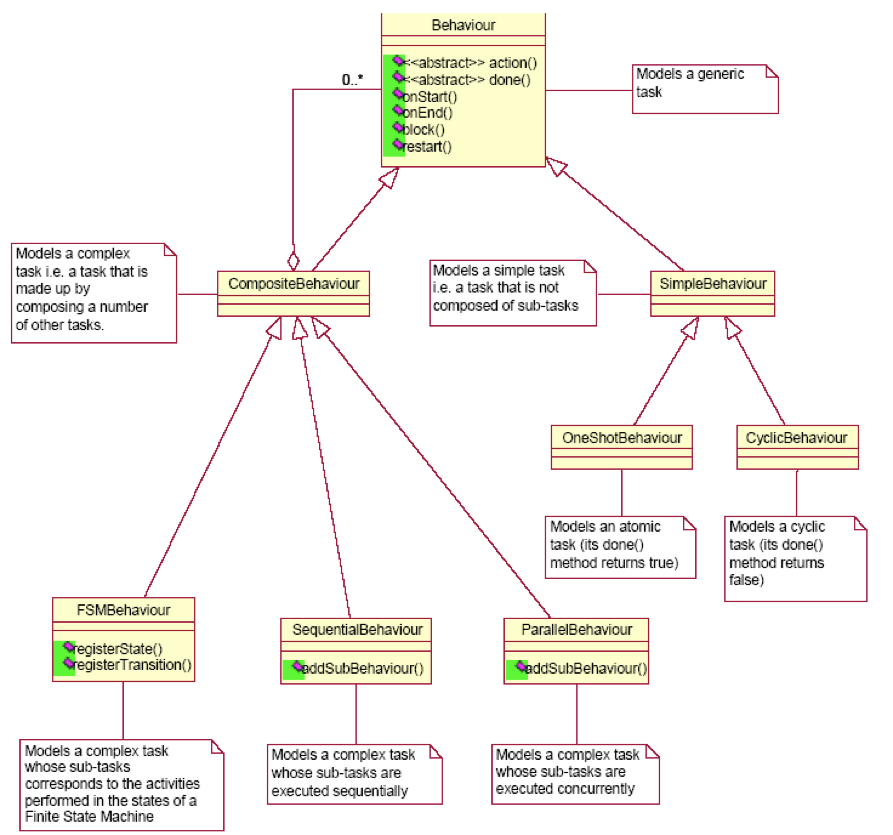
\includegraphics[width=.65\textwidth]{res/img/jade_behaviour_uml}
    \end{center}
    %
\end{frame}
%\\\\\\\\\\\\\\\\\\\\\

%\\\\\\\\\\\\\\\\\\\\\
\begin{frame}[c,allowframebreaks]\frametitle{\texttt{Behaviour} API}
    %
    \begin{block}{\texttt{jade.core.behaviours}}
        \emph{All behaviours} are in package \alert{\texttt{jade.core.behaviours}}
    \end{block}
    %
    \bigskip
    %
    \begin{block}{\texttt{SimpleBehaviour}}
        %
        \begin{itemize}
            \item \alert{\texttt{OneShotBehaviour}}
            %
            \begin{itemize}
                \item method \texttt{action()} is executed only once\ldots
                \item \ldots hence, method \texttt{done()} always returns \texttt{true}
            \end{itemize}
            %
            \item \alert{\texttt{CyclicBehaviour}}
            %
            \begin{itemize}
                \item method \texttt{done()} always returns \texttt{false}\ldots
                \item \ldots hence, method \texttt{action()} is executed forever---until agent death
            \end{itemize}
            %
        \end{itemize}
        %
    \end{block}
    %
    \begin{block}{\texttt{CompositeBehaviour}: sequential vs.\ parallel}
        %
        \begin{itemize}
            \item \alert{\texttt{SequentialBehaviour}}
            %
            \begin{itemize}
                \item method \texttt{addSubBehaviour()} to add \emph{child} behaviours\ldots
                \item \ldots to be scheduled \emph{sequentially}---method \texttt{done()} drives progress
                \item the whole behaviour ends when the last child ends
            \end{itemize}
            %
            \item \alert{\texttt{ParallelBehaviour}}
            %
            \begin{itemize}
                \item method \texttt{addSubBehaviour()} to add \emph{child} behaviours\ldots
                \item \ldots to be scheduled \emph{concurrently}
                \item two termination conditions provided by default---through constants
                %
                \begin{itemize}
                    \item \texttt{WHEN\_ALL} children are \texttt{done}
                    \item \texttt{WHEN\_ANY} child is \texttt{done}
                \end{itemize}
                %
                other conditions may be implemented by the programmer exploiting \jade{} API---see \texttt{checkTermination()} method
            \end{itemize}
            %
        \end{itemize}
        %
    \end{block}
    %
    \begin{block}{\texttt{CompositeBehaviour}: FSM}
        %
        \begin{itemize}
            \item \alert{\texttt{FSMBehaviour}}
            %
            \begin{itemize}
                \item method \texttt{registerState()} to add a child behaviour to the FSM
                %
                \begin{itemize}
                    \item each child represents the activity to be performed within a state of the FSM
                \end{itemize}
                %
                \item method \texttt{registerTransition()} to add a transition
                %
                \begin{itemize}
                    \item the value returned by the \texttt{onEnd()} \emph{callback} method is used to select the transition to fire
                \end{itemize}
                %
                \item some of the children can be registered as \emph{final states}\ldots
                \item \ldots hence, the whole behaviour terminates after the completion of any of them
            \end{itemize}
            %
        \end{itemize}
        %
    \end{block}
    %
    \begin{block}{Other behaviours}
        Many other very useful abstract behaviours exist, such as
        %
        \begin{itemize}
            \item \texttt{WakerBehaviour}
            %
            \begin{itemize}
                \item methods \texttt{action()} and \texttt{done()} are already implemented, so to execute abstract method \texttt{onWake()} when specified, then terminate
            \end{itemize}
            %
            \item \texttt{TickerBehaviour}
            %
            \begin{itemize}
                \item methods \texttt{action()} and \texttt{done()} are again already implemented, so to execute abstract method \texttt{onTick()} periodically as specified, then terminate when abstract method \texttt{stop()} is called
            \end{itemize}
            %
            \item \ldots
        \end{itemize}
        %
        Please refer to the \jade{} Programmer's Guide for the others \ccite{jade-progguide4}
    \end{block}
    %
\end{frame}
%\\\\\\\\\\\\\\\\\\\\\

%\\\\\\\\\\\\\\\\\\\\\
\begin{frame}\frametitle{Behaviours Scheduling: Recap}
    %
    \begin{center}
        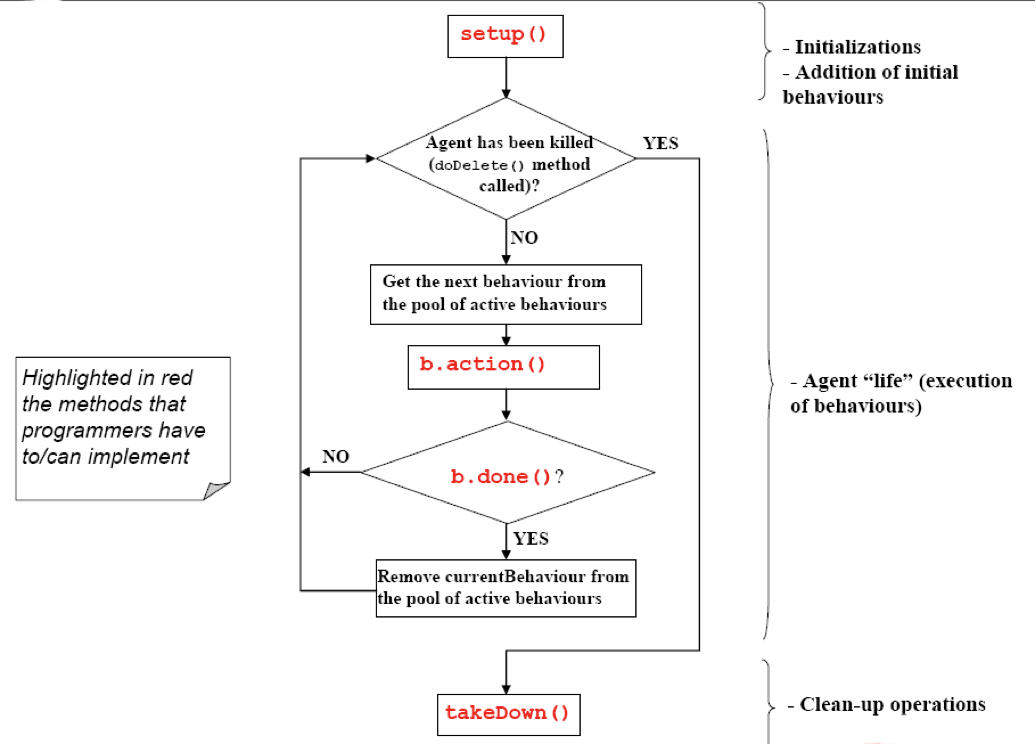
\includegraphics[width=.75\textwidth]{res/img/jade_behaviour}
    \end{center}
    %
\end{frame}
%\\\\\\\\\\\\\\\\\\\\\

%\\\\\\\\\\\\\\\\\\\\\
\begin{frame}[c,allowframebreaks]\frametitle{Round-Robin, Non-Preemptive Scheduling}
    %
    \begin{block}{The \texttt{setup()} method}
        By overriding the \texttt{setup()} method, \jade{} programmers ensure their agents have an initial pool of \emph{ready-to-schedule} behaviours
        %
        \begin{itemize}
            \item method \texttt{addBehaviour()} to add a behaviour (also usable elsewhere)
            \item method \texttt{removeBehaviour()} to remove one (better use it elsewhere\ldots)
        \end{itemize}
        %
        \texttt{setup()} serves to create instances of these behaviours and \emph{link} them to the owner agent
    \end{block}
    %
    \begin{block}{Round-robin}
        After initialisation, first behaviour from the \emph{active behaviours} pool (\alert{ready queue}) is scheduled for execution
    \end{block}
    %
    \begin{block}{Some remarks}
        %
        \begin{itemize}
            \item[!] behaviours switch occurs only when the \texttt{action()} method of the currently scheduled behaviour returns
            %
            \begin{itemize}
                \item[$\rightarrow$] hence, when it is running \emph{no other behaviour can execute}
            \end{itemize}
            %
            \item[!] behaviour removal from the scheduler pool occurs only when \texttt{done()} returns \texttt{true}
            %
            \begin{itemize}
                \item[$\rightarrow$] thus, if it returns \texttt{false} the behaviour is re-scheduled for next \emph{round}
            \end{itemize}
            %
            \item[!] \texttt{action()} is run \emph{from the beginning every time}: there is no way to ``stop-then-resume'' a behaviour
            %
            \begin{itemize}
                \item[$\rightarrow$] therefore, the computational state must be explicitly managed by the programmer in instance variables% (or exploiting \texttt{CompositeBehaviour})
            \end{itemize}
            %
        \end{itemize}
        %
    \end{block}
    %
    \begin{block}{One more remark}
        %
        \begin{itemize}
            \item programmers may need their agents to wait for something to happen---typically, a message to arrive
            \item programmers may be lured to use method \texttt{doWait()} for the purpose\ldots
            \item[!] \ldots don't do it!
            %
            \begin{itemize}
                \item[!] \texttt{doWait()} moves the agent to the WAITING state, where none of its behaviours can be executed!
            \end{itemize}
            %
            \item[$\rightarrow$] use method \alert{\texttt{block()}} provided by any behaviour class instead, which allows to \emph{suspend only the calling behaviour}
            %
            \begin{itemize}
                \item[$\rightarrow$] as soon as \texttt{action()} returns, the behaviour is moved to a special queue of blocked behaviours\ldots
                \item[$\rightarrow$] \ldots from which can be restored in the ready queue \emph{whenever any message arrives} or by explicitly calling \texttt{restart} method
            \end{itemize}
            %
        \end{itemize}
        %
    \end{block}
    %
\end{frame}

%\begin{frame}[c]
%    \frametitle{Examples in \texttt{ds.lab.jade.behaviours.*}}
%    Open a command prompt and position yourself into folder \cterm{ds-jade/}
%    \begin{itemize}
%        \item \cterm{java -cp libs/jade.jar:bin/ jade.Boot -gui -agents ste:ds.lab.jade.behaviours.SimpleBehavioursAgent}
%        \item \cterm{java -cp libs/jade.jar:bin/ jade.Boot -gui -agents ste:ds.lab.jade.behaviours.CompositeBehavioursAgent}
%        \item \cterm{java -cp libs/jade.jar:bin/ jade.Boot -gui -agents ste:ds.lab.jade.behaviours.FSMLikeAgent}
%    \end{itemize}
%    On Windows, substitute ``:'' with ``;'', and ``/'' with ``\textbackslash''
%\end{frame}
%\\\\\\\\\\\\\\\\\\\\\

%-------------------------------------------------------------------------------
\subsection{\jade{} Messaging}
%-------------------------------------------------------------------------------

%%\\\\\\\\\\\\\\\\\\\\\
\begin{frame}[c,allowframebreaks]\frametitle{More on \acl{} Messages}
    %
    \begin{block}{\fipa{} performatives}
        \alert{Performatives} identify the type of \emph{communicative act} carried out by the message---thus its semantics and expected response
        %
        \begin{description}
            \item[\texttt{CFP}] (Call For Proposal) to obtain proposals about something
            \item[\texttt{INFORM}] to let someone know something
            \item[\texttt{PROPOSE}] to propose something
            \item[\texttt{REQUEST}] to ask for a service
            \item[\texttt{SUBSCRIBE}] to subscribe for notification about something
            \item[\texttt{AGREE}] to express consensus about something
            \item[\texttt{REFUSE}] to refuse a request
            \item[\ldots] \ldots
        \end{description}
        %
        They are constants to be set for any \acl{} message exchanged by agents
    \end{block}
    %
    \begin{block}{\fipa{} message syntax}
        The syntax of an \acl{} message is defined by \fipa{} to enable interoperability
        %
        \begin{description}
            \item[\texttt{addReceiver()}] to add a value to the \texttt{:receiver} slot
            \item[\texttt{setContent()}] to fill in the \texttt{:content} slot
            \item[\texttt{setConversationId()}] to fill in the \texttt{:conversation-id} slot
            \item[\texttt{setEncoding()}] to fill in the \texttt{:encoding} slot
            \item[\texttt{setInReplyTo()}] to fill in the \texttt{:in-reply-to} slot
            \item[\texttt{setLanguage()}] to fill in the \texttt{:language} slot
            \item[\texttt{setOntology()}] to fill in the \texttt{:ontology} slot
            \item[\texttt{setSender()}] to fill in the \texttt{:sender} slot
            \item[\ldots] \ldots
        \end{description}
        %
    \end{block}
    %
\end{frame}
%\\\\\\\\\\\\\\\\\\\\\

%-------------------------------------------------------------------------------
\subsection{\jade{} Communication API}
%-------------------------------------------------------------------------------

%\\\\\\\\\\\\\\\\\\\\\
\begin{frame}[c,allowframebreaks]\frametitle{Agents Communication Basics}
    %
    \begin{block}{Sending messages}
        In order to send a message, an agent should
        %
        \begin{enumerate}
            \item create an \acl{} message
            %
            \begin{itemize}
                \item \footnotesize\texttt{ACLMessage msg = new ACLMessage(ACLMessage.<performative>);}
            \end{itemize}
            %
            \item fill its (mandatory) fields
            %
            \begin{itemize}
                \item \footnotesize\texttt{msg.addReceiver(new AID(receiver));}
                \item \footnotesize\texttt{msg.setContent("<content>");}
                \item \ldots
            \end{itemize}
            %
            \item call the \texttt{send()} method
            \begin{itemize}
                \item \footnotesize\texttt{send(msg);}
            \end{itemize}
        \end{enumerate}
        %
    \end{block}
    %
    \begin{block}{Replying to messages}
        In order to simplify answering, the \texttt{ACLMessage} class provides method \texttt{createReply()} to automatically set a number of \acl{} fields
        %
        \begin{itemize}\begin{small}
                \item \texttt{:receiver}
                \item \texttt{:language}, \texttt{:ontology}
                \item \texttt{:conversation-id}, \texttt{:protocol}
                \item \texttt{:in-reply-to}, \texttt{:reply-with}
        \end{small}\end{itemize}
        %
        Anyway, the programmer is free to overwrite such slots
    \end{block}
    %
    \begin{block}{Who to talk with?}
        %
        \begin{itemize}
            \item[?] how to find agents to talk to?
            \item when sending messages we must know the receiver \texttt{AID}
            %
            \begin{itemize}
                \item[$\rightarrow$] should we necessarily know it at compile-time?
            \end{itemize}
            %
            \item[!] \jade{} provides several ways to get an agent ID:
            %
            \begin{itemize}
                \item by using the agent \alert{local name} (whenever known)
                \item from the RMA GUI
                \item by asking to the AMS
                \item by asking to the DF (we'll see how to next lesson)
            \end{itemize}
            %
        \end{itemize}
        %
    \end{block}
    %
    \begin{block}{\jade{} local names}
        The simplest way to identify an agent is by its local name
        \begin{itemize}\tt
            \item[]\ldots
            \item[] msg.addReceiver(new AID("myAgent", \alert{AID.ISLOCALNAME}));
            \item[] \ldots
        \end{itemize}
        \jade{} ACC will automatically associate to the given agent name its \texttt{AID}
    \end{block}
    %
    \begin{block}{\jade{} RMA}
        By simply launching the RMA with
        \begin{center}
            \texttt{java -cp \ldots{} jade.Boot \alert{-gui}}
        \end{center}
        you have a GUI which displays all agents in the monitored \jade{} platform along with their \texttt{AID}s
    \end{block}
    %
    \begin{block}{Using the AMS}
        A much more comprehensive and flexible way to query \jade{} about existing agents is by interacting with the AMS service
        %
        \begin{enumerate}
            \item prepare a placeholder for agents with\\\begin{small}\texttt{\alert{AMSAgentDescription} [] agents = null;}\end{small}
            \item configure some kind of ``template'' on agents with\\\begin{small}\texttt{AMSAgentDescription template = new AMSAgentDescription (\ldots);}\end{small}
            \item configure search parameters with\\\begin{small}\texttt{\alert{SearchConstraints} c = new SearchConstraints(\ldots);}\end{small}
            \item launch the search process with\\\begin{small}\texttt{agents = \alert{AMSService.search}(this, template, c);}\end{small}
            \item collect AIDs with\\\begin{small}\texttt{AID aid = agents[i].\alert{getName()};}\end{small}
        \end{enumerate}
        %
    \end{block}
    %
\end{frame}
%\\\\\\\\\\\\\\\\\\\\\

%\\\\\\\\\\\\\\\\\\\\\
\begin{frame}[c,allowframebreaks]\frametitle{More on Agents Communication}
    %
    \begin{block}{\jade{} communication primitives}
        %
        \begin{description}
            \item[\texttt{send()}] to \alert{asynchronously send} a message---recipient is implicit
            \item[\texttt{receive()}] to \alert{asynchronously retrieve} the first message from the mailbox (if any)
            \item[\texttt{receive(MessageTemplate)}] to perform a \emph{selective receive}
            \item[\texttt{blockingReceive()}] to perform a \emph{synchronous} receive
            \item[\texttt{blockingReceive(long)}] to perform a \emph{timed} synchronous receive
            \item[\texttt{blockingReceive(MessageTemplate)}] to perform a selective, synchronous receive
            \item[\texttt{blockingReceive(MessageTemplate, long)}] to perform a timed, selective, synchronous receive
        \end{description}
        %
    \end{block}
    %
    \begin{block}{Receiving messages}
        One need to be careful when receiving messages
        %
        \begin{itemize}
            \item[!] method \texttt{blockingReceive()} \emph{suspends all agent behaviours}, not only the calling one---due to synchronicity
            %
            \begin{itemize}
                \item[$\rightarrow$] call \texttt{receive()} then \texttt{block()} instead, so to resume the behaviour whenever any message arrives
                \item[$\rightarrow$] call \texttt{blockingReceive()} only when you actually need to suspend all behaviours---e.g. during \texttt{setup()}
            \end{itemize}
            %
            \item[!] method \texttt{receive()} \emph{removes} the first message from the mailbox, therefore it may ``steal'' someone else's
            %
            \begin{itemize}
                \item[$\rightarrow$] use \alert{\texttt{jade.lang.acl.MessageTemplate}} within a \texttt{receive()} to get only messages \emph{matching a given pattern}
            \end{itemize}
            %
        \end{itemize}
        %
    \end{block}
    %
    \begin{block}{Selective receive}
        \texttt{jade.lang.acl.MessageTemplate} allows \jade{} agents to perform receive operations only \emph{on a subset of their mailbox}, which is the subset with only those messages \alert{matching} the given template
    \end{block}
    %
    \begin{block}{Hint}
        When a \jade{} agent is required to have \emph{parallel negotiations} with several other agents, one should
        %
        \begin{itemize}
            \item create a \texttt{:conversation-id} string to \emph{uniquely} identify messages
            \item by using the proper \texttt{MessageTemplate}, set up a behaviour which only responds to messages with that particular \texttt{:conversation-id}
        \end{itemize}
        %
    \end{block}
    %
    \begin{block}{\texttt{MessageTemplate} API I}
        A set of static, \emph{factory methods} are provided to build different kinds of template objects
        %
        \begin{description}
            \item[\texttt{matchAll()}] matches any \acl{} message
            \item[\texttt{matchContent()}] match checked on \texttt{:content} slot
            \item[\texttt{matchCustom(ACLMessage)}] template built so to match the given \acl{} message
            \item[\texttt{matchConversationId()}] match checked on \texttt{:conversation-id} slot
            \item[\texttt{matchOntology()}] match checked on \texttt{:ontology} slot
            \item[\texttt{matchSender()}] match checked on \texttt{:sender} slot
            \item[\ldots] \ldots
        \end{description}
        %
    \end{block}
    %
    \begin{block}{\texttt{MessageTemplate} API II}
        \ldots along with elementary boolean operators to combine them into more complex patterns\ldots
        %
        \begin{description}
            \item[\texttt{and()}] to build a template which is the \emph{intersection} of two given templates
            \item[\texttt{or()}] to build a template which is the \emph{union} of two given templates
            \item[\texttt{not()}] to build a template which is the \emph{negation} of a given template
        \end{description}
        %
        \ldots{} and a non-static method to actually check matching
        %
        \begin{description}
            \item[\texttt{match(ACLMessage)}] returns \texttt{true} if the given message matches the template upon which it is called
        \end{description}
        %
    \end{block}
    %
\end{frame}

%\begin{frame}[c, allowframebreaks]
%    \frametitle{Examples in \texttt{ds.lab.jade.messaging.*}}
%    Open a command prompt and position yourself into folder \cterm{ds-jade/}
%    \begin{itemize}
%        \item \cterm{java -cp libs/jade.jar:bin/ jade.Boot -gui -agents ste:ds.lab.jade.messaging.PingPongAgent}
%        \begin{itemize}
%            \item from RMA GUI launch the ``DummyAgent''
%            \item right-click on blank text field next to ``Receivers'' and left-click ``Add''
%            \item check ``NAME'' checkbox and digit ``ste'' (or whichever name you gave to he ping pong agent) then ``Ok''
%            \item select ``propose'' as the ``Communicative act'' and fill ``Content'' with either ``ping'' or ``pong''
%            \item fill ``Ontology'' with ``ping-pong''
%            \item click ``Send'' (envelope icon)
%            \item select messages from the box on the right (most recent at the top) and click ``View'' (glasses icon) to inspect message content
%        \end{itemize}
%    \end{itemize}
%    On Windows, substitute ``:'' with ``;'' an ``/'' with ``\textbackslash''
%    \begin{itemize}
%        \item \cterm{java -cp libs/jade.jar:bin/ jade.Boot -gui -agents calculator:ds.lab.jade.messaging.calculator.CalculatorAgent \&} (agent name MUST BE ``calculator'')
%        \item \cterm{java -cp libs/jade.jar:bin/ jade.Boot -container -agents ste:ds.lab.jade.messaging.calculator.ClientAgent \&}
%    \end{itemize}
%    On Windows, substitute ``\&'' with ``start /B'' (placed as first command)
%\end{frame}
%\\\\\\\\\\\\\\\\\\\\\

\section{Operations}

\subsection{\jade{} + Gradle}

\begin{frame}{Running \jade{} from Gradle}

    We provide two tasks for running \jade{} from Gradle:
    %
    \vfill
    %
    \begin{itemize}
    	\item \alert{\texttt{startPlatform}} --- creates \& starts a new platform with GUI
    	%
    	\begin{itemize}
    		\item default name: \texttt{it.unibo.sd.jade.platform}
    		%
    		\begin{itemize}
				\item (settable through the \texttt{platformName} property)
    		\end{itemize}

    		\item default host: \texttt{localhost}
    		%
    		\begin{itemize}
    			\item (settable through the \texttt{platformHost} property)
    		\end{itemize}

    		\item \alert{no agent} further agent is instantiated
    	\end{itemize}

    	\vfill

	    \item \alert{\texttt{startContainer}} --- creates \& starts a new container
	    %
	    \begin{itemize}

	    	\item default name: \texttt{it.unibo.sd.jade.container\#\textit{TIMESTAMP}}
	    	%
	    	\begin{itemize}
	    		\item (settable through the \texttt{containerBaseName} property)
	    	\end{itemize}

	    	\item assumes a platform is running on \texttt{localhost}
	    	%
	    	\begin{itemize}
	    		\item (different hosts can be provided via the \texttt{platformHost} property)
	    	\end{itemize}

    		\item agents to be instantiated can be specified via the \alert{\texttt{agents}} property
    		%
    		\begin{itemize}
    			\item semi-colon-separated list of string in the form
    			%
    			\begin{center}\ttfamily
    				AGENT\_NAME\alert{:}package.of.AgentClass$\underbrace{\texttt{(arg1, arg2, \ldots)}}_{optional}$
    			\end{center}
    		\end{itemize}
	    \end{itemize}
    \end{itemize}
\end{frame}

\begin{frame}{General workflow for demos}

	\begin{enumerate}
		\item Start a new, empty platform with
		%
		\begin{itemize}
			\item[\$] \texttt{gradle startPlatform}
		\end{itemize}

		\vfill

		\item Edit the code of the agent to be discussed (e.g. \texttt{HelloAgent})

		\vfill

		\item Add the following line to \texttt{gradle.properties}:
		%
		\begin{center}\ttfamily
			\alert{agents}=\textit{helloAgent}:it.unibo.ds.jade.HelloAgent
		\end{center}

		\vfill

		\item Start a new container containing the \texttt{helloAgent} agent
		%
		\begin{itemize}
			\item[\$] \texttt{gradle startContainer}
		\end{itemize}

		\vfill

		\item Inspect the logs, draw conclusions

		\vfill

		\item Close the container $\rightarrow$ Change some code $\rightarrow$ Restart container

		\vfill

		\item Close the platform

	\end{enumerate}

 \end{frame}

\section{Demos}

\begin{frame}{Agents' code overview}
	\lstinputlisting[language=Java]{./res/src/ExampleAgent.java}
\end{frame}

\startDemo

\subsection{Demo \currentDemo{} -- Atomic actions}

\begin{frame}{Demo \currentDemo{} -- Hello World}
	\lstinputlisting[language=Java]{./res/src/HelloAgent.java}
	%
	\begin{itemize}
		\item what do you expect the agent to do?
	\end{itemize}
\end{frame}

\begin{frame}{Demo \currentDemo{} -- One-Shot Behaviour}

	A behaviour which is executed just once:
	%
	\vfill
	%
	\lstinputlisting[language=Java]{./res/src/OneShotBehaviour.java}
	%
	\begin{itemize}
		\item represents \alert{atomic} actions
	\end{itemize}
\end{frame}

\startDemo

\subsection{Demo \currentDemo{} -- Long-lasting actions}

\begin{frame}{Demo \currentDemo{} -- Hello World\textbf{s}}
	\lstinputlisting[language=Java]{./res/src/HelloAgent2.java}
	%
	\begin{itemize}
		\item what do you expect the agent to do?
	\end{itemize}
\end{frame}

\begin{frame}{Demo \currentDemo{} -- Cyclic Behaviour}

	A behaviour which is executed infinitely many times:
	%
	\vfill
	%
	\lstinputlisting[language=Java]{./res/src/CyclicBehaviour.java}
	%
	\begin{itemize}
		\item represents \alert{long-lasting} actions
		\item what's the advantage w.r.t. ordinary \texttt{while(true)} loops?
	\end{itemize}
\end{frame}

\startDemo

\subsection{Demo \currentDemo{} -- Advantages of Internal Scheduling}

\begin{frame}[allowframebreaks]
    \frametitle{Demo \currentDemo{} -- Concurrent behaviours}

    Consider the following agent:
    %
    \lstinputlisting[language=Java]{./res/src/HelloAgent3.java}

    \bigskip

    What do you expect the agent to do?
    %
    \begin{itemize}
        \item positive number first? why?
        \item negative number first? why?
        \item some \alert{interleaving} of positive and negative numbers? which one?
    \end{itemize}

    \framebreak

    \begin{block}{Round-robin cooperative scheduling}
        An agent can carry out \alert{several} behaviours \alert{simultaneously}
        %
        \begin{itemize}
            \item behaviours run concurrently

            \item using a \alert{Round-Robin}, cooperative policy
            %
            \begin{itemize}
                \item[!] deterministic
                \item interleaving occurs at the \texttt{action()} level
            \end{itemize}

            \item 1-agent-1-thread
            %
            \begin{itemize}
                \item[$\rightarrow$] behaviours share the same thread
                \item[$\rightarrow$] the agent is always executing at most 1 \texttt{action()} at a time
            \end{itemize}
        \end{itemize}
    \end{block}

    \framebreak

    Expected outcome:
    %
    \lstinputlisting{./res/src/ExpectedOutcome3.txt}

    \framebreak

    Pay attention to the \alert{cooperative} part. Consider for instance:
    %
    \lstinputlisting[language=Java]{./res/src/HelloAgent4.java}

    \bigskip

    \begin{alertblock}{Avoid \textbf{long-standing} tasks within behaviours}
        \begin{itemize}
            \item they would block/slow down any other behaviour
            \item and therefore the whole agent
        \end{itemize}
    \end{alertblock}

\end{frame}

\section{API}

\subsection{Disclaimer}

\begin{frame}\frametitle{About \jade{} API}
    \begin{itemize}
        \item \jade{} was firstly implemented when Java was a far simpler language
        %
        \begin{itemize}
            \item no generics, no lambdas, no asynchronous programming
        \end{itemize}

        \vfill

        \item currently it is not actively maintained
        %
        \begin{itemize}
            \item a lot of legacy code is still there
            \item perfectly working, yet old fashioned
        \end{itemize}

        \vfill

        \item thus \jade{} code can easily become really verbose

        \vfill

        \item to mitigate this issue our first exercises focus on building a modern API for behaviours

        \vfill

        \item this will ease the creation of complex behaviours in the future
        %
        \begin{itemize}
            \item other than letting you practice with \jade{} agents' programming
        \end{itemize}
    \end{itemize}
\end{frame}

\subsection{The \texttt{Behaviours} class}

\begin{frame}[allowframebreaks]\frametitle{The \texttt{Behaviour\textbf{s}} class}
    Class full of \alert{static factory methods}\footnote{\url{https://en.wikipedia.org/wiki/Factory_method_pattern}} for most common behaviours:
    %
    \begin{description}
        \item[\texttt{atomic(Runnable)}] --- creates a \texttt{OneShotBehaviour} out of a lambda expression
        \item[\texttt{sequence(Behaviour,Behaviour...)}] --- creates a \texttt{SequentialBehaviour} out of a number of behaviours
        \item[\texttt{all(Behaviour,Behaviour...)}] --- creates a \texttt{ParallelBehaviour} out of a number of behaviours, requiring \alert{all} of them to terminate before terminating
        \item[\texttt{any(Behaviour,Behaviour...)}] --- creates a \texttt{ParallelBehaviour} out of a number of behaviours, requiring \alert{any} of them to terminate before terminating
        \item[\texttt{stop()}] --- creates a \texttt{ParallelBehaviour} out of a number of behaviours, requiring \alert{any} of them to terminate before terminating
    \end{description}
\end{frame}



%===============================================================================
\section*{}
%===============================================================================
\frame{\titlepage}

%%===============================================================================
%\section*{\bibname}
%%===============================================================================
%
%\setbeamertemplate{page number in head/foot}{}
%%\\\\\\\\\\\\\\\\\\\\\
%\begin{frame}[t,allowframebreaks,noframenumbering]\frametitle{\refname}
%    % \begin{frame}[c]\frametitle{\refname}
%    %	\footnotesize
%    %	\scriptsize
%    \tiny
%    \bibliographystyle{plain}
%    \bibliography{sd-lab-jade}
%\end{frame}
%%\\\\\\\\\\\\\\\\\\\\\

%%%%%%%%%%%%%%%%%%%%%%%%%%%%%%%%%%%%%%%%%%%%%%%%%%%%%%%%%%%%%%%%%%%%%%%%%%%%%%%
\end{document}
%%%%%%%%%%%%%%%%%%%%%%%%%%%%%%%%%%%%%%%%%%%%%%%%%%%%%%%%%%%%%%%%%%%%%%%%%%%%%%%%
